\documentclass[12pt]{article}
\usepackage[a4paper, hmargin={2.8cm, 2.8cm}, vmargin={2.5cm, 2.5cm}]{geometry}
\usepackage{eso-pic} % \AddToShipoutPicture

\usepackage[utf8]{inputenc}
\usepackage[T1]{fontenc}
\usepackage{lmodern}
\usepackage[english]{babel}
\usepackage{cite}
\usepackage{amssymb}
\usepackage{amsfonts}
\usepackage{amsmath}
\usepackage{enumerate}
\usepackage{mathrsfs}
\usepackage{fullpage}
\usepackage[linkcolor=red]{hyperref}
\usepackage[final]{graphicx}
\usepackage{color}
\usepackage{listings}
\renewcommand*\lstlistingname{Code Block}
\definecolor{bg}{rgb}{0.95,0.95,0.95}

%caption distinct from normal text
\usepackage[hang,small,bf]{caption}
\usepackage{hyperref}

\hypersetup{
    colorlinks,%
    citecolor=black,%
    filecolor=black,%
    linkcolor=black,%
    urlcolor=black
}

\author{
  \texttt{Gruppe: 3D} \\
  \texttt{Mikkel Enevoldsen} \\[.4cm]
  \texttt{Kristian Høi} \\[.4cm]
  \texttt{Dominique Chancelier} \\[.4cm]
  \texttt{Carsten Jensen} \\[.4cm]
  Instruktor: Jesper Lundsgaard
  \vspace{8cm}
}

\title{
  \vspace{3cm}
  \Huge{Opgave 5} \\[.25cm]
  \large{Kontekstuel Analyse}
  \vspace{.75cm}
}

\begin{document}

\AddToShipoutPicture*{\put(0,0){\includegraphics*[viewport=0 0 700 600]{includes/ku-farve}}}
\AddToShipoutPicture*{\put(0,602){\includegraphics*[viewport=0 600 700 1600]{includes/ku-farve}}}

%% Change `ku-en` to `nat-en` to use the `Faculty of Science` header
\AddToShipoutPicture*{\put(0,0){\includegraphics*{includes/ku-en}}}

\clearpage\maketitle
\thispagestyle{empty}

\newpage

\tableofcontents %generate table of content

\thispagestyle{empty}

\newpage
\pagestyle{plain}
\setcounter{page}{1}
\pagenumbering{arabic}

\section{Fremgangsmåde}
noget om pact\\
noget om tjekliste til interview\\
Vores generelle fremgangsmåde var at, gennemføre en brainstorm og itnerviews før vi begyndte at definere hvad vores fiva app præcist skulle kunne. Til vores interview udarbejdede vi en tjekliste, hvorpå vi havde en strukturet fremgangsmåde under de interviews.\\

Med henblik på interviews fandt vi vores deltager på gaden, hvor vi spurgte handlede ved supermarkeder hvor vi spurgte dem om det fremtidige system.\\
Kønsopdelingen for interviewdeltagerne er 3 mænd og 3 kvinder. nedenunder:
\begin{center}
    \begin{tabular}{ | l | l | l | l |}
    \hline
    \textbf{Køn} & \textbf{alder} & \textbf{uddannelse} & \textbf{Arbejde}\\ \hline
    Mand & 67 & Kok & pensionist \\ \hline
    Kvinde & 31 & RUC & Journalist \\ \hline
    Mand & 68 & Klejnsmed & pensionist \\ \hline
    Kvinde & 23 & Medie-videnskab & studerende \\ \hline
    Mand & 19 & HTX & studerende \\ \hline
    Kvinde & 41 & Erhversøkonomi og mediekutlur & Vi skal finde på noget her :) \\ \hline
     \end{tabular}
\end{center}
På baggrund af interviews og brainstorming kunne vi begynde at udforme hvilke funktioner vores system skulle ud og hvilke hensyn vi skulle tag til de fremtidige brugere af produktet.\\
På baggrund af vores analyse med interview og brainstorm udarbejde vi en målgruppe og to scenarier, hvor vi prøvede at forstille os et muligt forløb af interaktion mellem system og brugeren, hvor mest fokuserede på brugerens synsvinkel, da implementationsdetajler ikke kan laves på nuværende stadie\\
Tilsidst kunne vi lave vores papirs-prototype for at give os et overblik over
Til vores interview har vi spurgt seks personer. 
\newpage
\section{Resultat af indledende PACT-analyse}
Vi indlete projektet med, en omgang brainstorm med udgangs punkt i applictationen FIVA(Finde vare i supermarkedet), af den process fik vi 
en nogen stikord, som vi tog udgangspunkt i til bearbejdning af vores f\o rste interview tjekliste.
 
\textbf{People (Brugere)}
\begin{itemize} 
\item Sprogforskelle hvilke sprog synes vil v\ae re passende for FIVA
\item Hukommelse 
\item Generthed (sociale udfordringer ved henvendelse om vareplacering)
\item Socialklasser (indkomstforskelle)
\item Indkøbserfaring
\end{itemize}
Vi t\ae nkte p\aa hvilke sprog brugere vil synes det er passende for app'en, vi forrestillede os at appen kunne hj\ae lpe glemsemme bruger,
og bruger der generalt er sky, da det kan v\ae re gr\ae nse overkridende for dem at skulle sp\oe rg medarbejder om hj\ae lp. Vi legede ogsaa
med t\ae nken om socialklasser i det vi forstillede os at der nok er en bestem befolknings gruppe der vil benytte sig af app'en end andre.
Det var klar for os at potentiale brugere skulle have indk\o bserfaring og at app'en kunne forkorte noget af indsk\o bstiden.  

\textbf{Activity (Task, Opgaver)} 
\begin{itemize}
\item hyppighed 
\item Indkøbsfrekvens  
\item Tidspres
\item Formålet veldefineret: Handle ind.
\item Præventivt varetjek. 
\end{itemize}
Vi brainstormede med udgangspunkt i at den hovesagelige opgave er at k\o be ind, i den er der forbundet de forskelige aspekter, s\aa  som 
hvor mange gange en bruer handler om dagen, om det tit h\ae nger sammen med de har travlt. Vi havde en forstilling om at der m\aa ske var
nogen brugere der ringede ind for at h\o re om en bestem vare var p\aa  hylden f\o r de tog ned og handlede

\textbf{Context (Sammenh\ae ng, milj\o )}
\begin{itemize}
\item Supermarkeder - indk\o b
\end{itemize}
Det er meget relevant at bruger anvender FIVA appen i forbindelse med indk\o b i Supermarkeder, og det er \aa benlyst at supermarkeder
er milj\o en hvor app'en bruges. 

\textbf{Technology (Teknologi)}
\begin{itemize} 
\item GPS-tilgængelighed
\item Hurtighed
\item Højtlæsning af resultater
\end{itemize}
Den prim\ae re anvend teknologi er en Smartphone, og den har indbygget indbygget nogen features som kunne bruges i forbindelse med udvikling
af app'en. s\aa  som gps'en, app'en skal v\ae re hurtig og m\aa ske kunne h\o jste l\ae sning af resultater v\ae re til store gavn for nogle 
brugere. Vi t\ae nkte ogs\aa  at en tablet kunne bruges men det vil ikke v\ae re uden besv\ae r.   
\newpage

\section{Tjekliste til interview}
\textbf{Introduktion}\\
"Vi er datalogistuderende fra Københanvs Universitet, som skal designe en applikation omhandlende at gøre det lettere for kunden at finde varer. Vi ønsker at bruge 10 minutter på at få dine tanker omkring en sådan applikation  i et interview."
 
\begin{enumerate}
\item Fakta
\begin{enumerate}
\item Observér: Køn
\item Hvor gammel er du?
\item Hvilken teknologisk erfaring har du? Bruger du smartphone på daglig basis?
\end{enumerate}

\item Socialklasse "Hvilket erhverv og/eller uddannelsesbaggrund har du?"

\item Indkøbsfrekvens "Hvor tit handler du ind - og i hvilket tidsrum?"

\begin{enumerate}
\item Erfaring	"På hvilket niveau, erfaringsmæssigt, vil du beskrive dig selv som indkøber?"
\end{enumerate}

\item Tidsfaktor "Hvor lang tid har du til rådighed, når du handler ind?"
\item Motivation "Hvilken tilgang har du til indkøb - har du eksempelvis en struktureret plan over varer, eller køber du hvad der falder dig ind?"
\item Vareplacering "Fortæl mig om en situation, hvor du ikke har kunnet kunne finde en vare i et supermarked."

\begin{enumerate}
\item Hjælp "Hvor ofte må du spørge en medarbejder efter hjælp?"
\item Medarbejderfravær "Hvad gør du, når du ikke kan finde en varer og ikke kan komme i kontakt med en medarbejder?"
\end{enumerate}

\item Medarbejderkonfrontation "Hvilke udfordringer forbinder du med at skulle opsøge en medarbejder om en vares placering?"
\item Hukommelse "Hvor mange gange om måneden glemmer du hvad du skal købe i et supermarked? - Kan du fortælle om en specifik situation?"
\item Teknologisk vane "Hvis du har en smartphone, hvordan bruger du så den i forbindelse med indkøb?"

\begin{enumerate}
\item Teknologisk til-/fravalg "Hvorfor foretrækker du smartphone frem for andre alternativer?"
\end{enumerate}

\item Forberedelse "Hvordan forbereder du dig på en indkøbstur?"

\begin{enumerate}
\item Præventivt varetjek "Hvis vi kigger på de sidste 100 gange du har skullet købe ind, hvor mange gange vil du skyde på at du har ringer og spurgt i forvejen om de har en vare?"
\end{enumerate}

\item Forventning "Hvad ville du forvente en sådan applikation skulle indeholde? Og hvad må den absolut ikke indeholde?"
\item Hurtighed	"Hvor lang tid vil du sige, det højst burde tage at finde en vare ved hjælp af FIVA-appen, hvorfor?"
\item Sprogforskelle "Hvilket sprog synes du FIVA-appen skal være på?"
\item Nødvendighed "Ville du bruge en varelokaliserings-app til din smartphone, hvis sådan en fandtes - hvorfor?"

\begin{enumerate}
\item Alternativer "Kan du komme på alternativer, der ville gøre en sådan applikation overflødig?"
\end{enumerate}

\end{enumerate}

\section{Interviewresultater}
\subsection{Brugernes nuværende oplevelse}
\begin{enumerate}
\item Flere brugere er tidspressede når de skal handle ind, og oplever det derfor stressende, når det tager lang tid, som eksempelvis bruger () finder at det tager at finde specifikke varer.

\item Brugerne oplevede at hjælpen de fik, når de spurgte, ofte tog lang tid og til tidere var utilstrækkelig. Bruger (k,31) oplevede at medarbejder ikke kunne finde en varen og måtte tilkalde yderligere hjælp.

\item Brugere (1,2,3) finder relevansen af FIVA-appen til primært at være i supermarkeder, de ikke kender eller har handlet ind i før. De fleste kender placeringen på varerne i supermarkeder de tit kommer i.

\item Bruger (m,68)(k,31)(m,19)(m,67) fandt udfordringer med at konfrontere medarbejdere i forbindelse med placering på varer. Bruger (m,67)(m,68) fandt kontakt til medarbejdere besværlig, fandt dem svære at finde og ønskede ikke at spilde deres tid, mens bruger (k,31) vurderede der kunne være sproglige vanskeligheder hvis medarbejderne ikke taler dansk. Bruger (m, 19) fandt det akavet at spørge om hjælp. Kun en bruger (k, 41) sagde at hun ikke fandt nogen problemer med at spørge medarbejdere. De fleste (bruger 1, 2, 3, 4 og 6) sagde dog, at de på trods af disse udfordringer stadig opsøgte medarbejdere for at finde en vare, selvom det for brugers (()) vedkommende er en situation der kun sjældent forekommer.

\item Den generelle bruger (bruger (k,23)() ) skriver altid en indkøbsliste hjemmefra, som de bruger til at strukturere deres indkøb. Nogle specificerede dog yderligere, og bruger kun en liste ved større indkøbsture. Flere (bruger ()()) bruger ydermere i forvejen deres smartphone til at notere deres indkøbsliste ned på. 

\item Nogle brugere laver ugentligt mange små ture, hvor de kun køber få varer. Dette sker som oftest som konsekvens af tidligere glemt indkøb.

\item Nogle brugere strukturerer nøje deres indkøb efter andre daglige aktiviteter. Bruger (k,41) handler ind flere gange om dagen - en gang før hun afleverer børn i skole, og en gang på vej hjem fra at hente dem.
\end{enumerate}
\subsection{Forventning til appen}
\begin{enumerate}
\item Mange brugere (1,2,3) syntes at FIVA-appen skal kunne lokalisere varer og give de nødvendige direktioner hurtigt og effektivt. De fleste af dem (1,2) mener at det maksimalt må tage 30 sekunder at for appen at vise den korteste rute.

\item En bruger (1) mener at man skal kunne følge sin rute med en live GPS, i stil med den service Google maps eksempelvis tilbyder.\\

\item En bruger siger, at FIVA-appen skal være simpelt sat op og let at bruge. Bruger (1) mener yderligere at den skal indeholde et begrænset antal funktioner, for at gøre appen mere overskuelig og nemmere at arbejde med. 

\item Ifølge flere brugere, ville FIVA-appen skulle indeholde muligheden for at danne en indkøbsliste, og derved kombinere flere valgte varer og udregne en optimal rute for hele indkøbsturen.

\item En bruger (1) mener at appen, af overskuelighedsmæssige årsager, udelukkende skal være på dansk, mens flere andre brugere også synes at appen burde tilbydes på engelsk.

\item Det ville være forstyrende for flere brugere (1,2), hvis appen indeholdte udefrakommende reklamer.

\item En bruger (1) synes at man kunne give appen et socialt medie aspekt, således at brugerne skal kunne interagere med hinanden.

\item En bruger foreslog, at der kunne være en prissammenlignings mulighed inkluderet i appen, så hvis en vare skulle være billigere i et nærtliggende supermarked, skal appen gøre brugeren opmærksom på denne mulighed.

\item Flere brugere mener, at appen skal indeholde en søgefunktion, der når der søges efter varer, skal komme med søgeforslag efterhånden som der tastes ind. Den skal også kunne foreslå mere specifikke varer til en søgning.
\end{enumerate}

\section{Kerneopgaver}
Udfaldet af brainstorming og debat mellem gruppe deltager efter interviews b\o d dere efter p\aa nedst\aa ende  
\textbf{Interview}\\

\begin{enumerate}
\item Finde varer - Hylde nummer App'en skal kunne finde varen i butikken. Supermarked taster varens placering ind i deres system.
\item Tjekke om det er billigere hos nabobutikken. App'en skal kunne sammenligne priser på varer i en radius af 300 meter.
\item Søgefunktioner - Skal kunne hjælpe - Autocomplete. Den skal have en søgefunktion. Den skal kunne bidrage med yderligere hjælp, 
hvis kunden bare søger på vin. 
\item Simpel, minimalistisk, let at bruge.
\item Hurtig. Finde resultater indenfor max 10 sekunder. Skal kunne nortere en indkøbsliste.
\item Indkøbsliste. Lav optimal rute i supermarked. Simpel, minimalistisk, let at bruge. 
\end{enumerate}

\textbf{Gruppen}\\
\begin{enumerate}
\item Live gps - Giver rute hen til varen.
\item Nærmeste butik. Finder nærmeste supermarked.
\item Til kassen. Kortest vej til kassen. Der skal være en knap, så man hurtigt kan komme til kassen.Målgrupper:
\end{enumerate}
Primær målgruppe:
\begin{enumerate}
\item Smartphone-bruger der anvender den til simpelt brug, som ønsker at komme ubesværet igennem indkøb.

Sekund\ae r m\aa lgrupper
\item Vante smartphone-brugere, der ønsker at komme hurtigt igennem indkøb.
\item Vante smartphone-brugere, der handler ind til flere dage.
\item Smartphone-bruger der anvender den til simpelt brug, som ønsker at komme ubesværet igennem indkøb.
\item Prisbevidste folk der ønsker billigere varer
\end{enumerate}

\section{M\aa lgrupper og m\aa lgruppebeskrivelse}
\begin{itemize}
\item Kunder, der er vante smartphone-brugere, der ønsker at komme hurtigt igennem indkøb.
\item Kunder, der er vante smartphone-brugere, der handler ind til flere dage.
\item Kunder, der anvender smartphone til simpelt brug, som ønsker at komme ubesværet igennem indkøb.
\item Prisbevidste kunder der ønsker billigere varer.
\end{itemize}

\subsection{Målgruppebeskrivelse}
Målgruppen handler ind 3-4 gange om ugen. De ønsker en let og hurtig indkøbstur, hvor eventuelle problemer hurtigt ville kunne løses gennem FIVA-appen. De ønsker problemfrit at finde varer, som de sjældent køber.\\
Brugerne er vante indkøbere, og kender derfor det forventede varesortiment i butikken de ønsker at handle i.\\

\noindent Målgruppen bruger deres smartphones generelt til normal kommunikation, så som at ringe, sms og internetsøgninger. Brugeren ved hvad applikationer er, og bruger forbrugsapps, som eksempelvis Danske Banks mobilbank, Google Maps og Rejseplanen efter behov.\\

\noindent Målgruppen forstår at bruge en søgefunktion og følge en GPS' angivelser. De ved ikke hvordan smartphonen og appen fungerer internt. For dem er en smartphone, et redskab til at gøre hverdagen lettere.

\section{Personas}

\subsection{Lars Jensen}

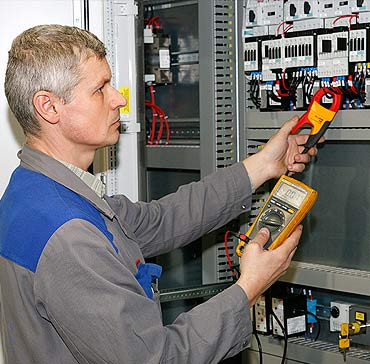
\includegraphics[scale=0.5]{includes/lars.jpg}
Lars Jensen er 57 år og bor i en forstad til Aarhus. Her han boet han sammen med sin kone, Lis Jensen, i de sidste 25 år. Sammen har de to børn, Michael på 18 og Anne på 21, der begge er flyttet hjemmefra.\\

\noindent Lars er uddannet elektriker, og har været vant til at gøre tingene selv i det meste af sit liv. Lars har haft en smartphone i omkring 2 år, og er ved at blive fortrolig med dens smarte funktioner.\\

\noindent Når der skal handles ind, er det oftest konen der sørger for det. Men desværre er Lis' hukommelse ikke hvad den har været, så derfor må Lars af og til ned og købe de enkelte ting hun glemmer. Han synes det er irriterende, at han så ofte må spørge medarbejdere om hjælp til at finde de forskellige varer. Han synes det spilder tiden for begge parter.

\subsection{Maria Møller}

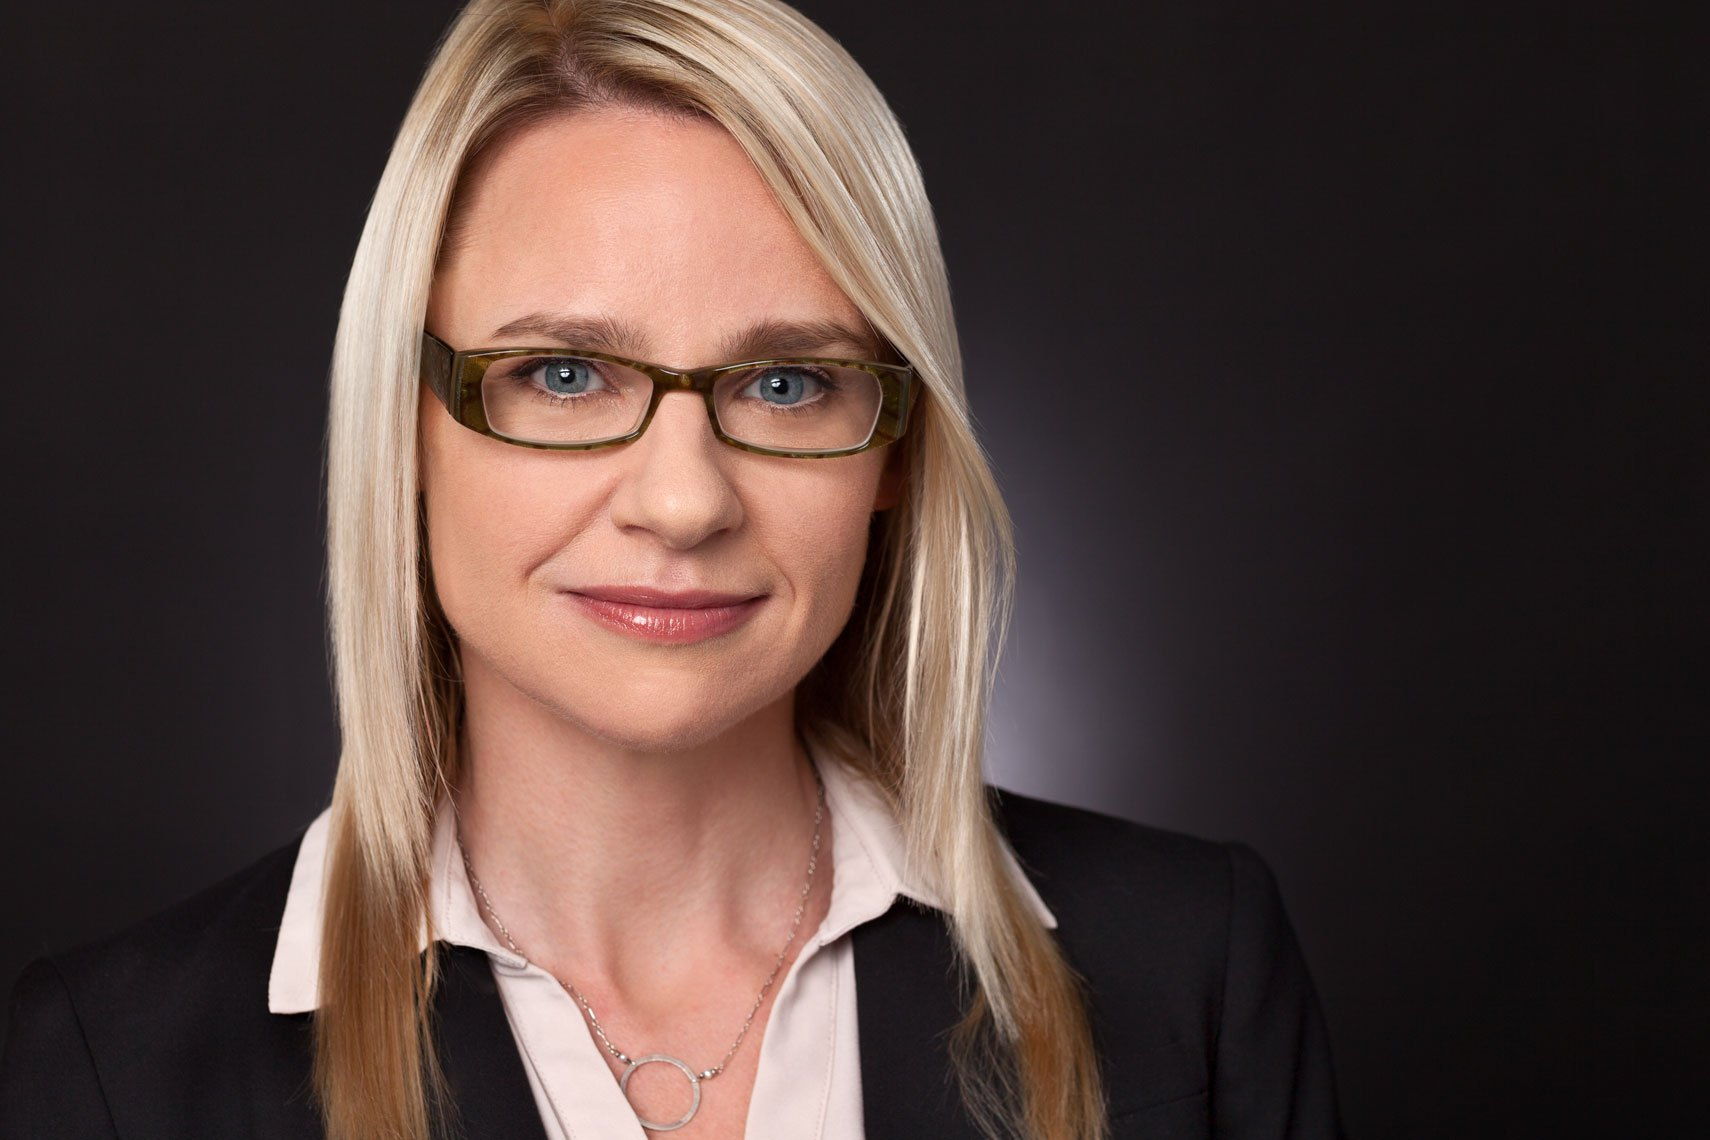
\includegraphics[scale=0.2]{includes/maria.jpg}
\noindent Maria Møller er 36 år og bor på Vesterbro i København. Hun bor sammen med sin søn, Emil, på 4 år. Maria er uddannet journalist på RUC, og er ansat på dagbladet Information. Hun har haft en smartphone i omkring 7 år og bruger den dagligt til at kommunikere med familie og venner samt tjekke nyheder.\\

\noindent Maria er glad for at udforske forskellige madkulturer, og hendes yndlingskøkkener er det asiatiske eller mexicanske. Dog har hun for nyligt begyndt at blive inspireret af det nynordiske køkken. Derfor handler hun mange forskellige og nye varer, som hun ikke altid ved hvor er i butikken. Derfor må hun ofte spørge medarbejderne om hjælp - og har oplevet flere gange, at de heller ikke ved hvor varen er.


\section{Scenarier}

\subsection{Lars Jensen}
Lars får at vide, at han skal ned og købe fennikel og kaffefiltre. Når Lars ankommer til supermarkedet åbner han sin nye FIVA-app og indtaster fennikel og kaffefilter i søgefunktionen. Lars har nu en rute, som han følger og finder sine varer. Han bruger "Gå til kassen"-funktionen, og får sin rute til kassen. Lars betaler, og skynder sig hjem.

\subsection{Maria Møller}
Maria sidder derhjemme og planlægger sin indkøbsliste. Her bruger FIVA-appen til at indskrive alle sine varer. Når Maria senere på dagen går ned for at handle, åbner hun appen og beder om ruten til sin indkøbsliste. Hun følger sin rute, men kommer undervejs i tanke om at hun også skal have artiskokker, som hun tilfældigvis ikke ved hvor ligger. Hun taster ind i appen, som tilpasser til hendes rute og viser placeringen på artiskokker. Hun finder sine artiskokker, og fortsætter sin rute.

\section{Prototype}

\section{Erfaringer}

\end{document}
